
\documentclass[tikz,border=5pt]{standalone}

% Core packages
\usepackage{amsmath,amssymb}
\usepackage{tikz}
\usepackage{tikz-cd}
\usepackage{pgfplots}
\usepackage{multicol}
\usepackage{xcolor}
\usepackage{caption}
\usepackage{float}
\usepackage{kotex}

% TikZ / PGF configuration
\usetikzlibrary{
  arrows.meta,
  calc,
  positioning,
  shapes.geometric,
  shapes.symbols,
  fit,
  backgrounds,
  patterns,
  matrix,
  intersections,
  decorations.pathmorphing,
  decorations.markings,
  angles,
  quotes
}
\pgfplotsset{compat=1.18}

% Reusable TikZ styles
\tikzset{
  >=stealth,
  line cap=round,
  line join=round,
  every picture/.style={line width=0.9pt},
  box/.style={draw, rounded corners, minimum width=2.8cm, minimum height=1.2cm, align=center},
  circlebox/.style={draw, circle, minimum size=1cm, align=center},
  arrow/.style={->, thick},
  dashedarrow/.style={->, thick, dashed},
  point/.style={circle, fill, inner sep=1.2pt},
  gridhelp/.style={help lines, gray!35},
  highlight/.style={fill=blue!10, draw=blue!60!black},
  3D/.style={
    x={(-0.60cm,-0.42cm)},
    y={(0.78cm,0cm)},
    z={(0cm,0.78cm)}
  }
}


\begin{document}

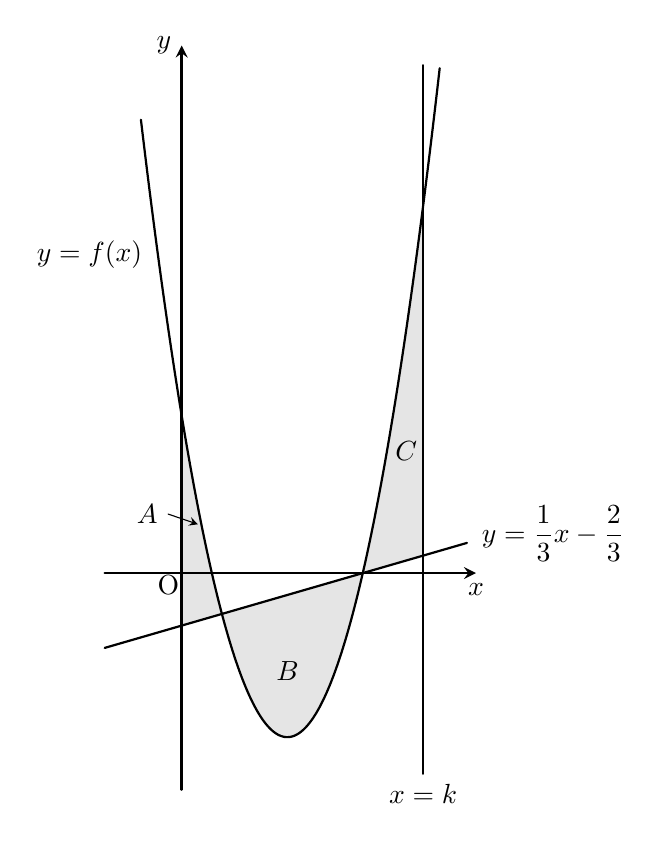
\begin{tikzpicture}[scale=1,
    x=1.15cm, y=1cm,
    line cap=round, line join=round,
    >=stealth
]
    \pgfmathsetmacro{\xone}{4/9}
    \pgfmathsetmacro{\xtwo}{2}
    \pgfmathsetmacro{\kval}{8/3}

    \fill[gray!20]
        (0,{0/3 - 2/3})
        -- (0,{3*0*0 - 7*0 + 2})
        -- plot[domain=0:\xone, samples=80, smooth, variable=\t]
            ({\t},{3*\t*\t - 7*\t + 2})
        -- plot[domain=\xone:0, samples=80, smooth, variable=\t]
            ({\t},{\t/3 - 2/3})
        -- cycle;
    \fill[gray!20]
        ({\xone},{\xone/3 - 2/3})
        -- plot[domain=\xone:\xtwo, samples=100, smooth, variable=\t]
            ({\t},{\t/3 - 2/3})
        -- plot[domain=\xtwo:\xone, samples=100, smooth, variable=\t]
            ({\t},{3*\t*\t - 7*\t + 2})
        -- cycle;
    \fill[gray!20]
        ({\xtwo},{3*\xtwo*\xtwo - 7*\xtwo + 2})
        -- plot[domain=\xtwo:\kval, samples=80, smooth, variable=\t]
            ({\t},{3*\t*\t - 7*\t + 2})
        -- plot[domain=\kval:\xtwo, samples=80, smooth, variable=\t]
            ({\t},{\t/3 - 2/3})
        -- cycle;

    \draw[->] (-0.85,0) -- (3.25,0) node[below] {$x$};
    \draw[->] (0,-2.75) -- (0,6.7) node[left] {$y$};
    \node[below left,yshift=1mm,xshift=1mm] at (0,0) {$\mathrm{O}$};

    \draw[thick, samples=180, smooth, variable=\t, domain=-0.45:2.85]
        plot ({\t},{3*\t*\t - 7*\t + 2});
    \draw[thick] (-0.85,{-0.85/3 - 2/3}) -- (3.15,{3.15/3 - 2/3});
    \draw[thick] (\kval,-2.55) -- (\kval,6.45);

    \node[left] at (-0.32,4.05) {$y=f(x)$};
    \node[right] at (3.2,0.5) {$y=\dfrac{1}{3}x-\dfrac{2}{3}$};
    \node[below] at (\kval,-2.55) {$x=k$};

    \node[left] (Alabel) at (-0.15,0.75) {$A$};
    \draw[->, thin] (Alabel.east) -- (0.18,0.62);
    \node at (1.17,-1.25) {$B$};
    \node at (2.48,1.55) {$C$};
 
\end{tikzpicture}

\end{document}

